\documentclass[conference]{IEEEtran}
\usepackage[utf8]{inputenc}
\usepackage[T1]{fontenc}
\usepackage[english]{babel}
\usepackage{amsmath,amssymb}
\usepackage{booktabs}
\usepackage{graphicx}
\usepackage{url}
\usepackage{hyperref}
\usepackage{tikz}
\usetikzlibrary{positioning,arrows.meta,shapes.geometric}
\usepackage{pgfplots}
\usepgfplotslibrary{groupplots}
\pgfplotsset{compat=1.18}

\begin{document}

\title{Sleep Quality, Social Jetlag, and Stress: An Observational Analysis of 69 Nights}

\author{\IEEEauthorblockN{Diego Arturo Almonte Villagómez}
\IEEEauthorblockA{Artificial Intelligence Engineering, Universidad Autónoma Chapingo, Texcoco, State of Mexico, Mexico.}}

\maketitle

\begin{abstract}
\textbf{Sleeping insufficiently on weekdays and attempting to recover on weekends is a widespread habit that often goes unnoticed until measured. In this report, I analyze my own sleep habits as an out-of-town Artificial Intelligence Engineering student with an academic routine marked by exams on Mondays, Wednesdays, and Fridays ($N=1$), across 69 consecutive nights recorded from 24/08/2026 to 31/10/2026: bedtime and wake-up time, total hours slept, sleep quality (1--10), nocturnal awakenings, pre-sleep smartphone use, exercise, and perceived stress (1--10). Sleep duration averaged $8.11\pm1.92$~h and quality averaged $7.00\pm1.46$; however, weekday sleep averaged $7.23\pm1.06$~h with a quality of $6.48\pm1.36$, whereas weekend sleep averaged $10.43\pm1.74$~h with a quality of $8.37\pm0.50$ ($p < 0.001$ in both cases), yielding a social jetlag of $1.97$~h (95\% CI: $1.41$--$2.50$). Sleep duration was the factor most strongly associated with quality (Spearman $\rho=0.77$; multiple regression: $+0.49$ points per hour, 95\% CI: $0.30$--$0.67$). Stress, nocturnal awakenings, and exercise showed no independent association; nights preceding exams did not differ from other weekday nights, and smartphone use before bed occurred on all 69 nights.}
\end{abstract}

\begin{IEEEkeywords}
Sleep quality, social jetlag, perceived stress, observational study, college students.
\end{IEEEkeywords}

\section{Introduction}

\subsection{Context and Problem}
Sleep is fundamental to human health. It has been proposed as a multidimensional construct encompassing duration, continuity, regularity, satisfaction, and daytime alertness~\cite{ref1}, with clinical guidelines recommending that adults obtain at least 7~h per night, within an optimal range of 7 to 9~h for young and middle-aged adults~\cite{ref2,ref3}. Improving sleep quality has been causally linked to better mental health in randomized controlled trials~\cite{ref4}.

University students represent a population characterized by irregular sleep schedules and multiple lifestyle disruptors~\cite{ref5,ref6}. As an out-of-town Artificial Intelligence Engineering undergraduate, I have weekly examinations on Mondays, Wednesdays, and Fridays (with Monday and Wednesday exams accounting for 100\% of the grade in their respective courses). Combined with exams, projects, and assignments from other subjects, this academic workload constitutes my primary source of stress. At the beginning of the observation period, I regularly attended the gym and basketball practice, but mounting academic demands and stress forced me to discontinue both. On weekdays, studying and completing assignments frequently push bedtime late into the night, resulting in sleep deprivation and poor rest, whereas weekends offer free time to sleep as much as possible. The core problem is that this irregular cycle substantially impairs physical and mental health, potentially leading to long-term consequences.

\subsection{Justification}
Self-tracking personal data is informative because population-level averages do not always reflect the reality of a specific individual. Analyzing 69 consecutive nights makes it possible to (i) quantify my exact sleep pattern and (ii) identify actionable associations within my own routine.

\subsection{Background}
The discrepancy between sleep schedules on workdays and free days generates social jetlag, defined as the difference between the midpoint of sleep on free days and on workdays~\cite{ref8}; in population data, social jetlag has been associated with a higher body mass index~\cite{ref9}. Electronic device use prior to sleep is associated with poorer sleep outcomes in recent meta-analyses (pooled correlation $r=0.28$, 95\% CI: $0.21$--$0.35$, for general use)~\cite{ref10}, and bedtime mobile phone use has been linked to sleep disturbances in adults~\cite{ref11}, mediated by underlying psychological processes~\cite{ref12,ref13}. Physical activity, smartphone usage, and perceived stress have been documented as key correlates of sleep quality among college students~\cite{ref14,ref15}; systematic reviews confirm the beneficial effects of exercise on sleep~\cite{ref16}, whereas psychosocial stress impairs it~\cite{ref17}. Evidence in adolescents similarly points to associations between screen exposure and sleep disruption~\cite{ref18,ref19}, though these population-based findings do not replace individualized self-assessment.

\subsection{Proposed Solution and Objectives}
To address this issue, I implemented a daily sleep log to reflect on empirical data and identify specific areas for improvement. \textbf{General objective:} to identify which recorded behavioral and contextual factors are associated with my sleep quality. \textbf{Specific objectives:} (1) describe overall sleep patterns; (2) compare weekdays against weekends and quantify social jetlag; (3) estimate associations between sleep quality and sleep duration, bedtime, nocturnal awakenings, stress, exercise, and smartphone use; and (4) propose a verification protocol tailored to my university schedule. \textbf{Hypotheses:} H1, sleep quality increases with sleep duration; H2, weekend sleep metrics differ significantly from weekday metrics; H3, physical exercise is associated with higher sleep quality; and H4, perceived stress is associated with lower sleep quality.

\section{Methodology}

\subsection{Design and Participant}
This is a longitudinal, single-subject ($N=1$) observational study with daily logging over 69 consecutive nights (Monday, 24/08/2026, through Saturday, 31/10/2026). Context: out-of-town Artificial Intelligence Engineering student with exams on Mondays, Wednesdays, and Fridays, alongside coursework from additional subjects, which led to discontinuing gym and basketball training due to academic workload.

\subsection{Variables and Instruments}
Table~\ref{tab:descriptiva} summarizes the recorded variables across the study period.

\begin{table}[ht]
\centering
\caption{Descriptive statistics ($n=69$ nights). Bedtime and wake-up time are expressed in 24-hour format.}
\label{tab:descriptiva}
\resizebox{\columnwidth}{!}{%
\begin{tabular}{lcccc}
\toprule
\textbf{Variable} & \textbf{Mean (SD)} & \textbf{95\% CI} & \textbf{Median} & \textbf{Range} \\
\midrule
Sleep duration (h) & 8.11 (1.92) & 7.65--8.57 & 7.67 & 5.07--13.00 \\
Sleep quality (1--10) & 7.00 (1.46) & 6.65--7.35 & 7 & 3--9 \\
Awakenings & 0.29 (0.49) & 0.17--0.41 & 0 & 0--2 \\
Stress (1--10) & 7.48 (1.57) & 7.10--7.85 & 8 & 2--9 \\
Bedtime & 00:28 (1.16) & 00:11--00:45 & 00:00 & 22:00--03:00 \\
Wake-up time & 08:35 (1.79) & 08:09--09:01 & 07:40 & 07:00--13:00 \\
\midrule
Smartphone before bed & \multicolumn{4}{c}{69 of 69 nights (100\%)} \\
Physical exercise & \multicolumn{4}{c}{21 of 69 days (30.4\%)} \\
\bottomrule
\end{tabular}%
}
\end{table}

\subsection{Data Preparation and Validation}
Total sleep duration was computed from recorded bedtimes and wake-up times:
\begin{equation}
D_i = (t_i^{\text{wake}} - t_i^{\text{bed}}) \bmod 24
\end{equation}
To compute mean bedtimes accurately across midnight, timestamps occurring prior to 12:00 were shifted by adding 24~h (e.g., 00:30 became 24.5). The midpoint of sleep and social jetlag ($SJL$) were calculated as:
\begin{equation}
MS_i = t_i^{\text{bed}} + \frac{D_i}{2}, \qquad SJL = \overline{MS}_F - \overline{MS}_W
\end{equation}
where $F$ denotes free days (Saturday and Sunday) and $W$ denotes workdays (Monday through Friday). No missing values occurred across the dataset (69 of 69 nights complete). Fig.~\ref{fig:flujo_datos} illustrates the data collection and processing pipeline.

\subsection{Statistical Analysis}
Mean, standard deviation (SD), and 95\% confidence intervals (CI) based on the $t$-distribution are reported. Group comparisons were performed using the Mann-Whitney $U$ test (for ordinal or non-normally distributed variables) alongside Cohen's $d$ as a measure of effect size:
\begin{equation}
d = \frac{\overline{x}_1 - \overline{x}_2}{s_p}
\end{equation}
Associations with sleep quality were estimated via Spearman's rank correlation with 95\% bootstrap CIs (3,000 resamples), and through an ordinary least squares (OLS) multiple linear regression model:
\begin{equation}
Q_i = \beta_0 + \beta_1 D_i + \beta_2 S_i + \beta_3 W_i + \beta_4 E_i + \beta_5 B_i + \varepsilon_i
\end{equation}
where $Q$ denotes sleep quality, $D$ sleep duration, $S$ stress, $W$ nocturnal awakenings, $E$ exercise ($0/1$), and $B$ bedtime in hours past 00:00. Multicollinearity was evaluated using the variance inflation factor (VIF). The significance threshold was set at $\alpha=0.05$ without multiple-comparison adjustments, framing the analysis as exploratory.

\begin{figure}[htbp]
    \centering
    \resizebox{\linewidth}{!}{
    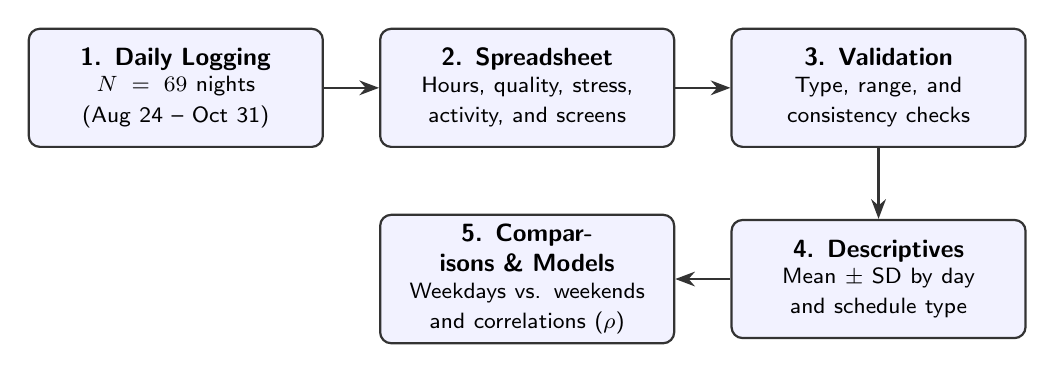
\begin{tikzpicture}[
        node distance=0.8cm and 0.7cm,
        caja/.style={
            rectangle, 
            rounded corners=4pt, 
            draw=black!80, 
            thick, 
            fill=blue!5, 
            text width=3.5cm, 
            minimum height=1.5cm, 
            align=center, 
            font=\small\sffamily
        },
        flecha/.style={
            -{Stealth[length=2.5mm]}, 
            thick, 
            draw=black!80
        }
    ]
        \node[caja] (n1) {\textbf{1. Daily Logging}\\ \footnotesize $N = 69$ nights\\(Aug 24 -- Oct 31)};
        \node[caja, right=of n1] (n2) {\textbf{2. Spreadsheet}\\ \footnotesize Hours, quality, stress,\\activity, and screens};
        \node[caja, right=of n2] (n3) {\textbf{3. Validation}\\ \footnotesize Type, range, and\\consistency checks};

        \node[caja, below=0.9cm of n3] (n4) {\textbf{4. Descriptives}\\ \footnotesize Mean $\pm$ SD by day\\and schedule type};
        \node[caja, left=of n4] (n5) {\textbf{5. Comparisons \& Models}\\ \footnotesize Weekdays vs. weekends\\and correlations ($\rho$)};

        \draw[flecha] (n1) -- (n2);
        \draw[flecha] (n2) -- (n3);
        \draw[flecha] (n3) -- (n4);
        \draw[flecha] (n4) -- (n5);
    \end{tikzpicture}%
    }
    \caption{Sleep data collection and analytical workflow ($N = 69$).}
    \label{fig:flujo_datos}
\end{figure}

\begin{figure}[h]
\centering
\fbox{\parbox{0.95\columnwidth}{
\footnotesize\ttfamily
\textbf{Algorithm 1: Analysis (All nights and Mon--Fri)}\\
1 \ read spreadsheet; keep rows with valid date\\
2 \ D <- (wake - bed) mod 24; verify vs log\\
3 \ bed\_c <- bed + 24 if bed < 12:00\\
4 \ MS <- bed\_c + D/2; SJL <- mean(MS|Sat,Sun) - mean(MS|Mon-Fri)\\
5 \ compute descriptives with 95\% CI (t)\\
6 \ Mann-Whitney U: Mon-Fri vs Sat-Sun; exercise Yes/No\\
7 \ Spearman(quality, x) + bootstrap CI\\
8 \ OLS(quality \textasciitilde{} hours+stress+awak+exer+bed)\\
9 \ repeat steps 6--8 for Mon-Fri only (n=50)\\
10 report effect sizes alongside p-values
}}
\end{figure}

\section{Results}

\subsection{Descriptive Statistics}
Table~\ref{tab:descriptiva} summarizes the 69 nights. Overall, 78\% of nights (54) achieved at least 7~h of sleep and 42 nights (61\%) fell within the recommended 7--9~h range, while 10 nights (14\%) lasted fewer than 6~h. At least one nocturnal awakening was recorded on 19 nights. Smartphone usage prior to sleep occurred on all 69 nights (100\%), and physical exercise was performed on 21 days (30.4\%). Fig.~\ref{fig:series} illustrates the daily time series.

\begin{figure*}[htbp]
\centering
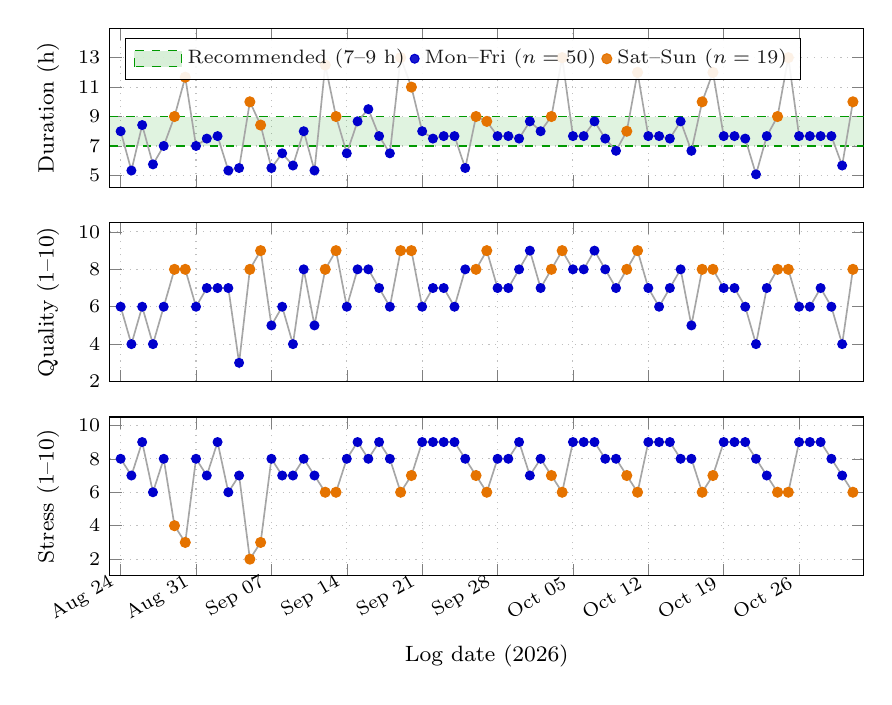
\begin{tikzpicture}
\begin{groupplot}[
    group style={
        group size=1 by 3,
        vertical sep=0.45cm,
        x descriptions at=edge bottom
    },
    width=0.92\textwidth,
    height=3.6cm,
    xmin=0, xmax=70,
    grid=both,
    grid style={dotted, gray!50},
    tick label style={font=\scriptsize},
    label style={font=\footnotesize},
    xtick={1, 8, 15, 22, 29, 36, 43, 50, 57, 64},
    xticklabels={Aug 24, Aug 31, Sep 07, Sep 14, Sep 21, Sep 28, Oct 05, Oct 12, Oct 19, Oct 26},
    xticklabel style={rotate=30, anchor=east}
]

% --- PANEL 1: SLEEP DURATION ---
\nextgroupplot[
    ylabel={Duration (h)},
    ymin=4.2, ymax=15.0,
    ytick={5, 7, 9, 11, 13},
    legend style={at={(0.02,0.94)}, anchor=north west, legend columns=3, font=\scriptsize, fill=white, fill opacity=0.9}
]
\addplot[draw=none, fill=green!60!black, fill opacity=0.12, forget plot] coordinates {(0,7) (70,7) (70,9) (0,9)};
\addplot[dashed, green!60!black, line width=0.6pt, forget plot] coordinates {(0,7) (70,7)};
\addplot[dashed, green!60!black, line width=0.6pt, forget plot] coordinates {(0,9) (70,9)};

\addplot[gray!70, line width=0.6pt, forget plot] coordinates {
(1,8.0) (2,5.33) (3,8.42) (4,5.75) (5,7.0) (6,9.0) (7,11.67) (8,7.0) (9,7.5) (10,7.67) (11,5.33) (12,5.5) (13,10.0) (14,8.42) (15,5.5) (16,6.5) (17,5.67) (18,8.0) (19,5.33) (20,12.5) (21,9.0) (22,6.5) (23,8.67) (24,9.5) (25,7.67) (26,6.5) (27,13.0) (28,11.0) (29,8.0) (30,7.5) (31,7.67) (32,7.67) (33,5.5) (34,9.0) (35,8.67) (36,7.67) (37,7.67) (38,7.5) (39,8.67) (40,8.0) (41,9.0) (42,13.0) (43,7.67) (44,7.67) (45,8.67) (46,7.5) (47,6.67) (48,8.0) (49,12.0) (50,7.67) (51,7.67) (52,7.5) (53,8.67) (54,6.67) (55,10.0) (56,12.0) (57,7.67) (58,7.67) (59,7.5) (60,5.07) (61,7.67) (62,9.0) (63,13.0) (64,7.67) (65,7.67) (66,7.67) (67,7.67) (68,5.67) (69,10.0)
};

\addlegendimage{area legend, fill=green!60!black, fill opacity=0.15, draw=green!60!black, dashed}
\addlegendentry{Recommended (7--9 h)}

\addplot[only marks, mark=*, mark size=1.6pt, blue!80!black] coordinates {
(1,8.0) (2,5.33) (3,8.42) (4,5.75) (5,7.0) (8,7.0) (9,7.5) (10,7.67) (11,5.33) (12,5.5) (15,5.5) (16,6.5) (17,5.67) (18,8.0) (19,5.33) (22,6.5) (23,8.67) (24,9.5) (25,7.67) (26,6.5) (29,8.0) (30,7.5) (31,7.67) (32,7.67) (33,5.5) (36,7.67) (37,7.67) (38,7.5) (39,8.67) (40,8.0) (43,7.67) (44,7.67) (45,8.67) (46,7.5) (47,6.67) (50,7.67) (51,7.67) (52,7.5) (53,8.67) (54,6.67) (57,7.67) (58,7.67) (59,7.5) (60,5.07) (61,7.67) (64,7.67) (65,7.67) (66,7.67) (67,7.67) (68,5.67)
};
\addlegendentry{Mon--Fri ($n=50$)}

\addplot[only marks, mark=*, mark size=1.8pt, orange!90!black] coordinates {
(6,9.0) (7,11.67) (13,10.0) (14,8.42) (20,12.5) (21,9.0) (27,13.0) (28,11.0) (34,9.0) (35,8.67) (41,9.0) (42,13.0) (48,8.0) (49,12.0) (55,10.0) (56,12.0) (62,9.0) (63,13.0) (69,10.0)
};
\addlegendentry{Sat--Sun ($n=19$)}

% --- PANEL 2: SLEEP QUALITY ---
\nextgroupplot[
    ylabel={Quality (1--10)},
    ymin=2, ymax=10.5,
    ytick={2, 4, 6, 8, 10}
]
\addplot[gray!70, line width=0.6pt, forget plot] coordinates {
(1,6) (2,4) (3,6) (4,4) (5,6) (6,8) (7,8) (8,6) (9,7) (10,7) (11,7) (12,3) (13,8) (14,9) (15,5) (16,6) (17,4) (18,8) (19,5) (20,8) (21,9) (22,6) (23,8) (24,8) (25,7) (26,6) (27,9) (28,9) (29,6) (30,7) (31,7) (32,6) (33,8) (34,8) (35,9) (36,7) (37,7) (38,8) (39,9) (40,7) (41,8) (42,9) (43,8) (44,8) (45,9) (46,8) (47,7) (48,8) (49,9) (50,7) (51,6) (52,7) (53,8) (54,5) (55,8) (56,8) (57,7) (58,7) (59,6) (60,4) (61,7) (62,8) (63,8) (64,6) (65,6) (66,7) (67,6) (68,4) (69,8)
};
\addplot[only marks, mark=*, mark size=1.6pt, blue!80!black] coordinates {
(1,6) (2,4) (3,6) (4,4) (5,6) (8,6) (9,7) (10,7) (11,7) (12,3) (15,5) (16,6) (17,4) (18,8) (19,5) (22,6) (23,8) (24,8) (25,7) (26,6) (29,6) (30,7) (31,7) (32,6) (33,8) (36,7) (37,7) (38,8) (39,9) (40,7) (43,8) (44,8) (45,9) (46,8) (47,7) (50,7) (51,6) (52,7) (53,8) (54,5) (57,7) (58,7) (59,6) (60,4) (61,7) (64,6) (65,6) (66,7) (67,6) (68,4)
};
\addplot[only marks, mark=*, mark size=1.8pt, orange!90!black] coordinates {
(6,8) (7,8) (13,8) (14,9) (20,8) (21,9) (27,9) (28,9) (34,8) (35,9) (41,8) (42,9) (48,8) (49,9) (55,8) (56,8) (62,8) (63,8) (69,8)
};

% --- PANEL 3: STRESS LEVEL ---
\nextgroupplot[
    ylabel={Stress (1--10)},
    xlabel={Log date (2026)},
    ymin=1, ymax=10.5,
    ytick={2, 4, 6, 8, 10}
]
\addplot[gray!70, line width=0.6pt, forget plot] coordinates {
(1,8) (2,7) (3,9) (4,6) (5,8) (6,4) (7,3) (8,8) (9,7) (10,9) (11,6) (12,7) (13,2) (14,3) (15,8) (16,7) (17,7) (18,8) (19,7) (20,6) (21,6) (22,8) (23,9) (24,8) (25,9) (26,8) (27,6) (28,7) (29,9) (30,9) (31,9) (32,9) (33,8) (34,7) (35,6) (36,8) (37,8) (38,9) (39,7) (40,8) (41,7) (42,6) (43,9) (44,9) (45,9) (46,8) (47,8) (48,7) (49,6) (50,9) (51,9) (52,9) (53,8) (54,8) (55,6) (56,7) (57,9) (58,9) (59,9) (60,8) (61,7) (62,6) (63,6) (64,9) (65,9) (66,9) (67,8) (68,7) (69,6)
};
\addplot[only marks, mark=*, mark size=1.6pt, blue!80!black] coordinates {
(1,8) (2,7) (3,9) (4,6) (5,8) (8,8) (9,7) (10,9) (11,6) (12,7) (15,8) (16,7) (17,7) (18,8) (19,7) (22,8) (23,9) (24,8) (25,9) (26,8) (29,9) (30,9) (31,9) (32,9) (33,8) (36,8) (37,8) (38,9) (39,7) (40,8) (43,9) (44,9) (45,9) (46,8) (47,8) (50,9) (51,9) (52,9) (53,8) (54,8) (57,9) (58,9) (59,9) (60,8) (61,7) (64,9) (65,9) (66,9) (67,8) (68,7)
};
\addplot[only marks, mark=*, mark size=1.8pt, orange!90!black] coordinates {
(6,4) (7,3) (13,2) (14,3) (20,6) (21,6) (27,6) (28,7) (34,7) (35,6) (41,7) (42,6) (48,7) (49,6) (55,6) (56,7) (62,6) (63,6) (69,6)
};

\end{groupplot}
\end{tikzpicture}
\caption{Nightly sleep duration, sleep quality, and perceived stress (blue: Monday to Friday; orange: Saturday and Sunday).}
\label{fig:series}
\end{figure*}

\subsection{Weekdays vs. Weekends}
On weekends, sleep duration was longer, quality was higher, and stress levels were lower (Table~\ref{tab:lv_sd}). Bedtime did not differ significantly ($p=0.52$); instead, the difference stemmed from wake-up time, which remained nearly constant on weekdays (07:36, SD 15~min) and shifted much later on weekends (11:11). Social jetlag reached $1.97$~h (95\% bootstrap CI: $1.41$--$2.50$), with sleep midpoints of 03:59 (Mon--Fri) and 05:57 (Sat--Sun). On weekdays, 15 of 50 nights (30\%) were shorter than 7~h, whereas 16 of 19 weekend nights (84\%) lasted 9~h or more. Moreover, 41 of 50 weekday nights (82\%) began after 00:00, and 16 (32\%) began after 01:00.

\begin{table}[h]
\centering
\caption{Monday--Friday ($n=50$) vs. Saturday--Sunday ($n=19$). Mean (SD); Mann-Whitney $U$ test.}
\label{tab:lv_sd}
\footnotesize
\begin{tabular}{lccc}
\toprule
\textbf{Variable} & \textbf{Mon--Fri} & \textbf{Sat--Sun} & \textbf{$p$} \\
\midrule
Sleep duration (h) & 7.23 (1.06) & 10.43 (1.74) & $<0.001$ \\
Sleep quality (1--10) & 6.48 (1.36) & 8.37 (0.50) & $<0.001$ \\
Awakenings & 0.28 (0.50) & 0.32 (0.48) & 0.69 \\
Stress (1--10) & 8.18 (0.87) & 5.63 (1.50) & $<0.001$ \\
Bedtime (hh:mm) & 00:22 & 00:44 & 0.52 \\
Wake-up time (hh:mm) & 07:36 & 11:11 & $<0.001$ \\
Exercise (days) & 19 (38\%) & 2 (11\%) & --- \\
\bottomrule
\end{tabular}
\end{table}

\subsection{Associations with Sleep Quality}
Sleep quality correlated strongly with sleep duration (Spearman $\rho=0.77$; Pearson $r=0.71$). Mean quality was $4.80$ for nights under 6~h ($n=10$), $6.00$ between 6 and 7~h ($n=5$), $6.84$ between 7 and 8~h ($n=25$), $7.75$ between 8 and 9~h ($n=12$), and $8.29$ for 9~h or more ($n=17$). Across all nights, stress and later bedtime showed moderate negative correlations with quality, although stress inverted its sign when restricted to weekdays (Table~\ref{tab:spearman}). Exercise showed no significant association with sleep quality: $6.76$ with exercise vs. $7.10$ without ($p=0.37$; $d=-0.23$), and $6.53$ vs. $6.45$ on weekdays ($p=0.88$).

The multiple regression model accounted for 52\% of the variance in sleep quality ($R_{\text{adj}}^2=0.48$; maximum VIF $= 1.92$). Only sleep duration exhibited an independent effect (Table~\ref{tab:ols}): each additional hour of sleep was associated with $+0.49$ quality points. Within weekdays alone, the slope increased to $0.83$ points per hour (95\% CI: $0.50$--$1.16$; $R_{\text{adj}}^2=0.49$). Because weekday wake-up times barely varied, bedtime largely determined total sleep duration ($\rho=-0.92$).

\begin{table}[h]
\centering
\caption{Spearman correlation with sleep quality [95\% bootstrap CI].}
\label{tab:spearman}
\resizebox{\columnwidth}{!}{%
\begin{tabular}{lcc}
\toprule
\textbf{Variable} & \textbf{All Nights ($n=69$)} & \textbf{Mon--Fri Only ($n=50$)} \\
\midrule
Sleep duration & $0.77$ [$0.63, 0.86$] & $0.59$ [$0.32, 0.80$] \\
Bedtime (later) & $-0.37$ [$-0.60, -0.11$] & $-0.61$ [$-0.81, -0.35$] \\
Stress & $-0.32$ [$-0.53, -0.06$] & $0.36$ [$0.08, 0.61$] \\
Awakenings & $-0.12$ [$-0.37, 0.14$] & $-0.29$ [$-0.53, 0.00$] \\
Exercise (yes) & $-0.11$ [$-0.35, 0.14$] & $0.02$ [$-0.29, 0.31$] \\
Weekend & $0.65$ [$0.52, 0.76$] & --- \\
\bottomrule
\end{tabular}%
}
\end{table}

\begin{table}[h]
\centering
\caption{Multiple linear regression predicting sleep quality ($n=69$, $R^2=0.52$).}
\label{tab:ols}
\resizebox{\columnwidth}{!}{%
\begin{tabular}{lccc}
\toprule
\textbf{Predictor} & \textbf{$\beta$} & \textbf{95\% CI} & \textbf{$p$} \\
\midrule
Intercept & $3.47$ & $0.64$--$6.29$ & $0.017$ \\
Sleep duration (per h) & $0.49$ & $0.30$--$0.67$ & $<0.001$ \\
Stress (per point) & $-0.04$ & $-0.25$--$0.17$ & $0.69$ \\
Awakenings (per event) & $-0.21$ & $-0.75$--$0.32$ & $0.43$ \\
Exercise (yes) & $0.07$ & $-0.51$--$0.64$ & $0.82$ \\
Bedtime (per h after 00:00) & $-0.14$ & $-0.42$--$0.15$ & $0.33$ \\
\bottomrule
\end{tabular}%
}
\end{table}

\subsection{Weekly Trends}
Perceived stress increased by $0.16$ points per week (linear regression, $p=0.018$), rising from a weekly mean of $6.4$ in Week 1 to $8.0$ in Week 10, whereas sleep quality and duration showed no significant linear trends ($p=0.26$ and $p=0.24$, respectively). Exercise frequency dropped from 3, 4, and 5 days during Weeks 1--3 (12 days total) to 2--3 days during Weeks 4--7 (9 days total), and zero sessions during Weeks 8--10; the final session occurred on 08/10/2026. This decline resulted directly from escalating stress and academic workload after that date, which led to abandoning physical training.

\section{Analysis and Discussion}

\paragraph{Sleep Duration and Quality (H1)}
The association between sleep duration and quality was the strongest finding, holding across all nights, within weekdays, in rank-order correlations, and in multiple regression. This aligns with the central role of duration within the sleep health framework~\cite{ref1}. Nevertheless, causal directionality cannot be strictly established: a poor night of rest may shorten or fragment sleep, and subjective quality is evaluated the following morning upon reflecting on how restorative the sleep felt alongside its length.

\paragraph{Weekends and Social Jetlag (H2)}
The weekday-to-weekend discrepancy was not driven by earlier bedtimes, but rather by waking up $3.6$~h later. A social jetlag of nearly 2~h falls within the threshold considered clinically relevant in the literature~\cite{ref8,ref9}. This pattern reflects accumulated weekday sleep debt (30\% of nights under 7~h) compensated during the weekend. Sleeping $10.4$~h on weekends is consistent with recovering lost rest from late-night study sessions. Furthermore, weekends alter multiple contextual variables simultaneously (lower stress, different activities), meaning ``weekend'' acts as an aggregate indicator.

\paragraph{Physical Exercise (H3)}
No statistically significant difference emerged between days with and without exercise, despite robust literature supporting its sleep benefits~\cite{ref16}. Because only 21 exercise days were logged—and none during the final three weeks—statistical power was limited. Dropping gym and basketball sessions due to academic workload and stress is clearly captured in the dataset, with zero sessions recorded after 08/10/2026. Thus, physical inactivity acted as a downstream consequence of academic pressure rather than an independent predictor. Although not reflected in nightly sleep scores, this lack of exercise noticeably affected my physical conditioning and daytime fatigue.

\paragraph{Perceived Stress (H4)}
The negative correlation observed across all nights (Table~\ref{tab:spearman}) disappeared after adjusting for sleep duration ($\beta=-0.04$) and inverted within weekdays ($\rho=0.36$). This represents a classic case of confounding by day type: stress peaks precisely on weekdays when sleep is shortest. Between Weeks 1 and 7, mean stress and quality rose together, whereas in Weeks 8--10 quality declined while stress remained elevated. The upward stress trajectory ($+0.16$/week) indicates that self-reported stress primarily captures academic load (exams plus assignments across all courses), which concurrently delays bedtime. The underlying pathway likely follows \textit{academic workload $\rightarrow$ late bedtime $\rightarrow$ shorter duration $\rightarrow$ lower sleep quality}: the data support this mechanism (on weekdays, bedtime explains nearly all variance in duration, $\rho=-0.92$), while self-reported stress compresses multiple stressors into a single metric.

\paragraph{Smartphone Usage}
Because pre-sleep smartphone use occurred every single night (100\%), its lack of variance precluded statistical comparison, though it likely depresses baseline sleep quality, consistent with prior literature~\cite{ref10,ref11,ref12}.

\paragraph{Action Hypothesis and Verification Protocol}
Advancing bedtime—given that wake-up time is constrained by morning classes (averaging 07:36)—is estimated to improve sleep quality by approximately $0.8$ points per hour (95\% CI: $0.50$--$1.16$). Moving average weekday bedtime 1~h earlier would shift it from 00:22 to roughly 23:20. Because late nights are driven by studying and coursework, this adjustment is only feasible by restructuring time management. I propose a 4-week $A/B$ self-experiment consisting of two baseline weeks followed by two intervention weeks incorporating: (i) a strict evening curfew for studying and assignments by shifting part of the workload to weekend hours, and (ii) two short exercise sessions per week to resume physical activity. The same variables will be logged alongside daily study hours and evening screen minutes, acknowledging that outcomes remain subject to the academic calendar.

\section{Conclusions and Future Work}
The findings of this 69-night self-tracking study reveal a notable paradox: the very period intended to monitor and improve my routine documented the abandonment of physical exercise and an increase in late-night study sessions driven by exams and assignments. Far from invalidating the role of exercise, the data confirm that the core bottleneck is not a lack of willpower, but the absence of structured time management capable of balancing university attendance, nutrition, physical activity, effective studying, and adequate rest.

At the same time, this analysis highlights practical constraints that govern behavioral change—most notably days with university schedules running from 08:00 to 18:00~h, after which mental exhaustion makes sustaining extracurricular routines difficult. As future work, I plan to structure a weekly schedule tailored to each day's class load, enforce a nightly cutoff for electronic screens, and maintain this sleep log to quantitatively evaluate the impact of these interventions on rest and stress levels.

\section*{AI Usage Disclosure}
An AI assistant (Gemini, Google, consulted November 8--15, 2026) was used for: (a) creating Fig.~1, (b) translating the manuscript into English, (c) proofreading spelling and grammar, and (d) formatting bibliographic references. All sleep records, personal and academic context, statistical interpretations, and conclusions are entirely my own.

\section*{Code and Data Availability}
The \LaTeX\ source code for this document, the statistical analysis scripts, and the 69-night dataset are publicly available at: \url{https://github.com/arturoalmonte82-cmyk/analisis-sue-o-69-noches#analisis-sue-o-69-noches}.

\begin{thebibliography}{19}

\bibitem{ref1} D. J. Buysse, ``Sleep health: can we define it? Does it matter?,'' \emph{Sleep}, vol. 37, no. 1, pp. 9--17, 2014.

\bibitem{ref2} M. Hirshkowitz et al., ``National Sleep Foundation's sleep time duration recommendations: methodology and results summary,'' \emph{Sleep Health}, vol. 1, no. 1, pp. 40--43, 2015.

\bibitem{ref3} N. F. Watson et al., ``Recommended amount of sleep for a healthy adult: a joint consensus statement of the American Academy of Sleep Medicine and Sleep Research Society,'' \emph{Sleep}, vol. 38, no. 6, pp. 843--844, 2015.

\bibitem{ref4} A. J. Scott, T. L. Webb, M. Martyn-St James, G. Rowse, and S. Weich, ``Improving sleep quality leads to better mental health: a meta-analysis of randomised controlled trials,'' \emph{Sleep Med. Rev.}, vol. 60, art. 101556, Dec. 2021.

\bibitem{ref5} H. G. Lund, B. D. Reider, A. B. Whiting, and J. R. Prichard, ``Sleep patterns and predictors of disturbed sleep in a large population of college students,'' \emph{J. Adolesc. Health}, vol. 46, no. 2, pp. 124--132, 2010.

\bibitem{ref6} S. D. Hershner and R. D. Chervin, ``Causes and consequences of sleepiness among college students,'' \emph{Nat. Sci. Sleep}, vol. 6, pp. 73--84, 2014.

\bibitem{ref7} V. Ibáñez, J. Silva, and O. Cauli, ``A survey on sleep assessment methods,'' \emph{PeerJ}, vol. 6, e4849, 2018.

\bibitem{ref8} M. Wittmann, J. Dinich, M. Merrow, and T. Roenneberg, ``Social jetlag: misalignment of biological and social time,'' \emph{Chronobiol. Int.}, vol. 23, no. 1--2, pp. 497--509, 2006.

\bibitem{ref9} T. Roenneberg, K. V. Allebrandt, M. Merrow, and C. Vetter, ``Social jetlag and obesity,'' \emph{Curr. Biol.}, vol. 22, no. 10, pp. 939--943, 2012.

\bibitem{ref10} X. Han, E. Zhou, and D. Liu, ``Electronic media use and sleep quality: updated systematic review and meta-analysis,'' \emph{J. Med. Internet Res.}, vol. 26, e48356, 2024, doi: 10.2196/48356.

\bibitem{ref11} L. Exelmans and J. Van den Bulck, ``Bedtime mobile phone use and sleep in adults,'' \emph{Soc. Sci. Med.}, vol. 148, pp. 93--101, 2016.

\bibitem{ref12} J. S. Peltz, J. S. Bodenlos, J. N. Kingery, and C. Abar, ``Psychological processes linking problematic smartphone use to sleep disturbance in young adults,'' \emph{Sleep Health}, vol. 9, no. 4, pp. 524--531, 2023.

\bibitem{ref13} M.-J. Kater and A. A. Schlarb, ``Smartphone usage in adolescents: motives and link to sleep disturbances, stress and sleep reactivity,'' \emph{Somnologie}, vol. 24, no. 4, pp. 245--252, 2020.

\bibitem{ref14} X. Zhai et al., ``Associations among physical activity and smartphone use with perceived stress and sleep quality of Chinese college students,'' \emph{Ment. Health Phys. Act.}, vol. 18, art. 100323, Mar. 2020.

\bibitem{ref15} M. Stanković, M. Nešić, S. Čičević, and Z. Shi, ``Association of smartphone use with depression, anxiety, stress, sleep quality, and internet addiction. Empirical evidence from a smartphone application,'' \emph{Pers. Individ. Differ.}, vol. 168, art. 110342, Jan. 2021.

\bibitem{ref16} M. A. Kredlow, M. C. Capozzoli, B. A. Hearon, A. W. Calkins, and M. W. Otto, ``The effects of physical activity on sleep: a meta-analytic review,'' \emph{J. Behav. Med.}, vol. 38, no. 3, pp. 427--449, 2015.

\bibitem{ref17} T. Åkerstedt, ``Psychosocial stress and impaired sleep,'' \emph{Scand. J. Work Environ. Health}, vol. 32, no. 6, pp. 493--501, 2006.

\bibitem{ref18} M. Hysing et al., ``Sleep and use of electronic devices in adolescence: results from a large population-based study,'' \emph{BMJ Open}, vol. 5, no. 1, e006748, 2015.

\bibitem{ref19} B. Carter, P. Rees, L. Hale, D. Bhattacharjee, and M. S. Paradkar, ``Association between portable screen-based media device access or use and sleep outcomes: a systematic review and meta-analysis,'' \emph{JAMA Pediatr.}, vol. 170, no. 12, pp. 1202--1208, 2016.

\end{thebibliography}

\end{document}
